\documentclass{article} % For LaTeX2e
\usepackage{iclr2026_conference,times}

% Optional math commands from https://github.com/goodfeli/dlbook_notation.
\input{math_commands.tex}

\usepackage{hyperref}
\usepackage{url}
\usepackage{graphicx}
\usepackage{subscript}
\usepackage[normalem]{ulem}
\usepackage{multirow}
\usepackage{pifont}
\usepackage{float}
\usepackage{xcolor}
\usepackage{amssymb}
\usepackage{booktabs}

\title{SpikeLoRA: Parametric Regularisation for Low-Rank Adaptation using Spiking Neural Networks}

% Authors must not appear in the submitted version. They should be hidden
% as long as the \iclrfinalcopy macro remains commented out below.
% Non-anonymous submissions will be rejected without review.

\author{Iwan de Jong, Anna S. Bosman, Andries Schreuder \\
Department of Computer Science\\
University of Pretoria\\
Pretoria, South Africa \\
\texttt{iwan.dejong@tuks.co.za,anna.bosman@up.ac.za,an.shreuder@up.ac.za} \\
}

% The \author macro works with any number of authors. There are two commands
% used to separate the names and addresses of multiple authors: \And and \AND.
%
% Using \And between authors leaves it to \LaTeX{} to determine where to break
% the lines. Using \AND forces a linebreak at that point. So, if \LaTeX{}
% puts 3 of 4 authors names on the first line, and the last on the second
% line, try using \AND instead of \And before the third author name.

\newcommand{\fix}{\marginpar{FIX}}
\newcommand{\new}{\marginpar{NEW}}

% \iclrfinalcopy % Uncomment for camera-ready version, but NOT for submission.
\begin{document}

\maketitle

\begin{abstract}
Low-rank adaptation (LoRA) is a fine-tuning method that freezes the parameters of a pre-trained model and injects small trainable matrices. Although LoRA has been widely used to efficiently fine-tune LLMs, it is susceptible to overfitting. To address this, we introduce SpikeLoRA, a spiking low-rank adaptation fine-tuning method that leverages the leaky integrate-and-fire (LIF) neuron to introduce learnable sparsity with minimal computational overhead. The LIF neuron acts as a gate to the activations from the \(A\)-matrix in LoRA, sparsifying activations while preserving learned information. This design makes SpikeLoRA an efficient and sparse fine-tuning method for both spiking and traditional LLMs when deployed on neuromorphic hardware. Our experiments show that it is possible to achieve up to 97.24\% learned sparsity without a substantial drop in evaluation metrics. 
% We also show that SpikeLoRA is able to outperform current regularisation techniques such as dropout (non-parametric) and gating (parametric).
\end{abstract}

\section{Introduction}
Fine-tuning forms part of the transfer learning domain \citep{raffel_exploring_2020}, and allows a pre-trained model to specialise in a downstream task, incorporating a specific domain of expertise, task, or knowledge. To achieve this, fine-tuning adjusts the weights of a pre-trained model to minimise some loss on a downstream task.%s better than a generic pre-trained model.

The problem with fine-tuning, however, is that parameters of the original model have to be updated (retrained). This results in computational inefficiencies and potential \emph{catastrophic forgetting}, where pre-trained knowledge may be lost \citep{song_how_2025}. Adapter modules, or adapters, were proposed as a solution to fine-tuning inefficiencies, and add small fully-connected networks on top of the frozen pre-trained parameters~\citep{houlsby_parameter-efficient_2019-1}. However, each downstream task requires its own adapter, making it difficult to switch tasks easily. Low-rank Adaptation (LoRA) is a novel fine-tuning approach which freezes the weights of the pre-trained model and uses low-rank matrix decomposition to parametrise the weight update \citep{hu_lora_2022}. This substantially reduces the trainable parameters, does not introduce any additional inference, and eliminates the need to calculate gradients for frozen parameters.

LoRA has evolved to multiple methods, including adaptive low-rank adaptation (AdaLoRA) \citep{zhang_adalora_2023-1}, adaptive learning low-rank adaptation (ALLoRA) \citep{huang_allora_2024}, weight-decomposed low-rank adaptation (DoRA) \citep{liu_dora_2024}, and quantised low-rank adaptation (QLoRA) \citep{dettmers_qlora_2023-1}, among others. These methods attempt to enhance LoRA's efficiency without compromising performance by introducing sparsification and quantisation techniques. Fundamentally, AdaLoRA dynamically adjust the rank of each respective LoRA module, ALLoRA eliminates dropout and scaling by introducing an adaptive learning rate, DoRA stabilises training by controlling weight redundancy, and QLoRA quantises the base model's weights while fine-tuning with LoRA. Furthermore, \citet{huang_allora_2024} investigated an adaptive scaling factor for LoRA (ASF-LoRA). Different from the constant scaling factor in \cite{hu_lora_2021}, ASF-LoRA makes the scaling factor trainable, but introduces potential ripple effects across layers, which degrade performance.

All of these LoRA variants operate on the model's weight matrices by optimising low-rank weight matrices for efficient fine-tuning. However, few widely used techniques are focused on the activations in the low-rank space. Dropout \citep{srivastava_dropout_2014} is a well-known regularisation method directed at the activations. Dropout stochastically zeroes activations during training to prevent co-adaptation of neurons. While dropout stochastically suppresses activations, a spiking neural network (SNN) offers promising characteristics to learn when to suppress activations.

SNNs are considered to be more biologically plausible neural networks, and make use of event-driven (discrete) spikes to transmit information \citep{singh_nebula_2020}. This makes SNNs sparse, which eliminates the need for continuous activations, as seen with ANNs. SNNs have been successfully utilised in spiking LLMs, such as SpikeGPT \citep{zhu_spikegpt_2024-1}. SNNs offer promising biologically-inspired capabilities and are more energy-efficient on specialised neuromorphic hardware. 
Since SNNs are sparse in nature, they possess the characteristics to learn when to sparsify activations, making them a viable option to act as a regulariser.
 %Due to their discrete event-driven nature, SpikeLoRA integrates the characteristics of an SNN into LoRA to sparsify activations, mitigate potential overfitting, and improve efficiency.

In this paper, we contribute the following:
\begin{enumerate}
  \item \textbf{SpikeLoRA:} A novel spiking version of LoRA is introduced, enabling more efficient fine-tuning on downstream tasks. By coupling the LoRA module with a leaky integrated-and-fire (LIF) neuron, biologically inspired parametric sparsification is introduced with minimal overhead. This allows SpikeLoRA to learn when to suppress activations while achieving comparable accuracy.
  % We aim to make SpikeLoRA part of the \texttt{PEFT}-repository\footnote{\url{https://github.com/huggingface/peft}} [pull request pending].
  \item \textbf{Application of LoRA and SpikeLoRA to SpikeGPT:} We fine-tune SpikeGPT \citep{zhu_spikegpt_2024-1} using both LoRA and SpikeLoRA to show the possibility and potential of LoRA in a full spiking pipeline. Coupled with SpikeLoRA, we make the entire fine-tuning process compatible with neuromorphic hardware.
\end{enumerate}

This paper is structured as follows: \textbf{Section \ref{background}} provides a background on the concepts used in this paper, including SpikeGPT and LoRA. \textbf{Section \ref{method}} introduces SpikeLoRA. \textbf{Section \ref{experiments}} discusses the experimental setup and results. \textbf{Section \ref{conclusion}} concludes the paper and outlines future work. %Finally, we include an appendix for additional details regarding our experiments.

\section{Background}
\label{background}
\subsection{Spiking Neural Network (SNN)}
\label{SNN}
Spiking Neural Networks (SNNs) are often referred to as the \emph{3rd generation of neural networks} \citep{capatina_efficient_2023,maass_networks_1997-1,yang_sdit_2024}. SNNs attempt to closely mimic the biological brain to solve known problems in deep learning, such as excessive memory usage, computational complexity \citep{eshraghian_training_2023-1}, and a lack of sufficient parallelism \citep{pfeiffer_deep_2018}. Memory usage is reduced by SNN's sparsity. Computational complexity is reduced when using bio-inspired spikes instead of continuous activations seen in ANNs. Parallelism is improved through the event-driven nature of an SNN.

SNN neurons are activated using binary inputs through time as inputs (known as a \emph{spike train}). An integrate-and-fire (IF) neuron uses these binary inputs and adds them to the current membrane potential. When the membrane potential reaches a pre-defined voltage threshold, the neuron fires. If not, the membrane potential will continue to build up until the voltage threshold is reached. If a neuron fires, it can contribute to the next neuron, but otherwise it acts as a silent neuron, which accounts for the sparsity of a spiking network. With the use of neuromorphic hardware, true sparsity and event-driven activations are prominent, such that silent neurons don't use any memory to store their activations.

\subsubsection{Leaky Integrate-and-Fire (LIF) Neuron}
While several neuron models exist, the intuitive first-order LIF neuron model has been widely used to understand SNNs \citep{kim_sharing_2023}, although incapable of efficiently learning long-term dependencies \citep{eshraghian_training_2023-1}. A first-order LIF neuron model \citep{dayan_theoretical_2001} comprises a couple of equations to perform activation for time step \(t\): \(V[t]\) (eq. \ref{eq:3}) and \(S[t]\) (eq. \ref{eq:4}). The function \(V[t]\) stores the membrane voltage potential of a neuron:
\begin{equation}\label{eq:3}
  % U[t] = H[t] + \beta (X[t] - (H[t-1] - U_{reset}))
  V[t] = \beta \cdot V[t-1] + W \cdot X[t] - S[t-1] \cdot V_{t}
\end{equation}
where \(\beta\) is a predefined decay factor (such as \(e^{-1/\tau}\) \citep{eshraghian_training_2023-1}) of \(V[t-1]\), the previous state of the neuron's membrane potential. \(\beta\) is used to simulate the leaky aspect of an IF neuron. If \(\beta = 1\), then equation \ref{eq:3} simply acts as a non-leaky IF neuron. \(W \cdot X[t]\) is the weighted input to the LIF-neuron. \(S[t-1]\) is a function to reset the membrane potential (eq. \ref{eq:4}). \(S[t] \in \{0,1\}\) since \(\Theta(\cdot) \in \{0,1\}\) (eq. \ref{eq:5}). Therefore \(V[t]\) causes the membrane potential (eq. \ref{eq:3}) to add up when the neuron is not fired (i.e. where \(V[t] < V_{t}\)) \citep{tavanaei_deep_2019-1}. When a neuron fires, \emph{reset-by-subtraction} will subtract the threshold, whereas \emph{reset-to-zero} will reset the membrane potential to zero \citep{eshraghian_training_2023-1}. The decision whether a neuron is fired or not is determined by \(S\) as follows:
\begin{equation}\label{eq:4}
  S[t] = \Theta (V[t] - V_{t})
\end{equation}
where \(\Theta\) is the Heaviside function \citep{legua_heaviside_2006}:
\begin{equation}\label{eq:5}
  \Theta(t) =
  \begin{cases}
    1 & t \geq 0 \\
    0 & t < 0
  \end{cases}
\end{equation}

For backpropagation, an arctangent surrogate gradient function has proven to be effective in approximating gradients, but it is unclear as to why this works so well \citep{eshraghian_training_2023-1}. The arctangent surrogate gradient solves the non-differentiable nature of the Heaviside function (eq. \ref{eq:5}). However, since these functions approximate gradients, a loss in performance can be expected \citep{pfeiffer_deep_2018}. A solution to compute gradients in SNNs is to set the final layer's voltage threshold extremely high so that the final neurons can't spike \citep{lee_enabling_2020-1}. To further enhance learning, \citet{fang_incorporating_2021} proposes a parametric LIF that introduces a learnable membrane time constant.

\subsection{SpikeGPT}
SpikeGPT \citep{zhu_spikegpt_2024-1}, a generative spike-based large language model (LLM), introduces a novel approach to replace traditional neurons in the receptance weighted key value (RWKV) architecture \citep{peng_rwkv_2023}, an alternative to the Transformer architecture, with spiking neurons. SpikeGPT is proven to be suitable for NLU and NLG tasks.

\label{srwkv} 
To avoid an additional dimension, \citet{eshraghian_training_2023-1} suggests adapting deep learning neurons with spiking thresholds in the attention head to learn long-term dependencies. SpikeGPT's novel Spiking RWKV \citep{zhu_spikegpt_2024-1} does something similar, but is instead inspired by RWKV. SRWKV employs the same foundation as RWKV's time-mixing block, but to be a spiking version, it also uses the recurrent properties of SNN. SWRKV unrolls the sequence \(X \in \mathbb{R}^{T \times d}\) to represent \(X[t] \in \mathbb{R}^{1 \times d}\). Similar to RWKV, SRWKV also use \(R\), \(K\), and \(V\) with linear transformations. These transformations are then used as inputs to the rest of the time-mixer block.

To adapt the FFN, found in the Transformer architecture \citep{vaswani_attention_2017}, to be a spiking NN, \citet{zhu_spikegpt_2024-1} propose a Spiking Receptance FFN (SRFFN). The SRFFN functions similarly to the channel mixer. This is coupled with a spiking gating mechanism. SRFFN contains learnable parameters and utilises LIF neurons as resulting outputs.

To build a spike train, SpikeGPT proposes binary embeddings (BE) to transform continuous outputs into binary spikes \citep{zhu_spikegpt_2024-1}. Although considered to be a spiking LLM, the binary embeddings only reside at the embedding layer, and fundamentally, SpikeGPT utilises continuous activations. This means that a LoRA module would still have to deal with continuous inputs and not binary embeddings.

\subsection{Low-Rank Adaptation (LoRA)}
\label{lora}

Formally, \(h\) as the output of the forward pass in a neural network with LoRA is defined as:
\begin{equation}\label{loraeq}
  h = W_0x + \Delta{W_x}
\end{equation}
where \(W_0x\) is the frozen weight matrix of \(x\). \(\Delta{W_x} = BA\) is the low-rank weight matrix where \(B \in \mathbb{R}^{d \times r}\) and \(A \in \mathbb{R}^{r \times k}\). The rank \(r\) must be less than \(d\) and \(k\). The forward pass of a network is calculated as usual, and during backpropagation, only the low-rank matrix is updated.

When fine-tuning with LoRA, new unseen dimensions, known as \emph{intruder dimensions}, can dominate the update, which could cause generalisation problems across domains \citep{shuttleworth_lora_2024}. These dimensions capture misleading correlations rather than learning generalisable features, which causes overfitting. On the other hand, it is also likely that, during fine-tuning, some features in \(\Delta{W}\) might be duplicated from \(W\), which can amplify important features \citep{hu_lora_2022}.

\section{SpikeLoRA Method}
\label{method}
\begin{figure}[ht!]
  \centering
  \includegraphics[scale=0.5]{assets/SpikeLoRA.png}
  \caption{High-level diagram of SpikeLoRA during forward pass. For illustration purposes, only a vector is shown as input. In practice, a multi-dimensional tensor is passed as input. Adapted from the original LoRA definition \citep{hu_lora_2022}.}
  \label{fig:SpikeLoRA}
\end{figure}

We aim to leverage the promising capabilities of SNNs and LoRA to potentially pave the way to fine-tune the next generation of neural networks and LLMs. SpikeLoRA, our proposed method, is based on the original LoRA definition \citep{hu_lora_2022} where \(\Delta W\) (Eq. \ref{loraeq}) is modified as:
\begin{equation}\label{LoRAeq}
  \Delta{W} = B \cdot ({\mathcal{SN}}(A) \odot A)
\end{equation}
where \({\mathcal{SN}}\) is the LIF neuron that takes \(A \in \mathbb{R}^{r\times k}\) as argument such that \({\mathcal{SN}}(A) = \text{LIF}(A) \in \{0,1\}^{r\times k}\). The element-wise product of the LIF node and the original down projection from \(A\) helps to preserve previously-learned information, while zeroing out elements corresponding to LIF nodes that did not spike (Fig. \ref{fig:SpikeLoRA}). In both traditional and current spiking LLMs \citep{zhu_spikegpt_2024-1}, the LIF neurons in the SpikeLoRA module learns through delta modulation, which is based on continuous activations rather than binary spike trains \citep{eshraghian_training_2023-1}.

In our design, each LoRA module is coupled with one LIF node, effectively gating the activations of the \(A\)-matrix (i.e., the \emph{adapter-in} matrix). Since the LIF node resides in the low-rank space of the LoRA module, the element-wise multiplication has an \(O(rk)\) complexity. When gating the \(B\)-matrix such that \({\mathcal{SN}}(B) = \text{LIF}(B) \in \{0,1\}^{d\times r}\), double-spiking occurs, which introduces possible downsides such as extreme sparsity. When gating \(BA\) (i.e. the \emph{adapter-out} matrix) of the module, the complexity increases to \(O(dk)\), since \(r \ll min(d,k)\) and \(BA \in \mathbb{R}^{d\times k}\).

Although SpikeLoRA could be considered a variation of LoRA, its cooperability with other variations is worth investigating \citep{zhao_merging_2025}. Since our modification of LoRA is primarily based on the addition of a LIF neuron, SpikeLoRA can easily be coupled with other LoRA variations, such as AdaLoRA \citep{zhang_adalora_2023-1}. Similar to dropout, SpikeLoRA doesn't directly affect the underlying mechanisms of those variations, allowing for efficient cooperability. For example, AdaLoRA's definition can be modified as:
\begin{equation}\label{LoRAeq}
  \Delta = ({\mathcal{SN}}(P) \odot P) \cdot \Lambda \cdot Q
\end{equation}
such that \({\mathcal{SN}}(P)\) is the spiking activation of the left singular vector \(P\). Additionally, other matrices can be experimented with as shown in \cite{lin_lora_2024-1}. For a method like AdaLoRA, it's important to mention that the forward pass is mostly trivial, while the backwards pass requires careful handling to avoid double-counting gradient modifications. It is possible to detach the LIF neuron from the graph, but this impacts its parametric nature.

\section{Experiments}
\label{experiments}
To evaluate SpikeLoRA, we divide our experiments into four sections:
\begin{enumerate}
    % \item \textbf{Univariate scaling analysis:} We perform a univariate scaling analysis to monitor the impact of SpikeLoRA's hyperparameters.
    \item \textbf{LoRA and SpikeLoRA on SpikeGPT:} SpikeGPT is fine-tuned using LoRA and the proposed SpikeLoRA module. We use the NLU results from \citet{zhu_spikegpt_2024-1} to perform a comparative performance analysis and show the potential of an efficient spiking fine-tuning pipeline.
    \item \textbf{SpikeLoRA on a traditional LLM:} DeBERTaV3-Base is fine-tuned using the proposed SpikeLoRA module. We explore various setups to assess the impact of hyperparameters. We use the GLUE \citep{wang_glue_2019-1} benchmark and compare SpikeLoRA directly to existing LoRA methods.
    \item \textbf{SpikeLoRA deep dive:} Smaller experiments are performed to evaluate SpikeLoRA's characteristics, such as energy efficiency, sparse dynamics, and ability to control overfitting. The position of the LIF node in the SpikeLoRA module is also experimented with.
\end{enumerate}
For SpikeGPT, we make use of existing benchmark results \citep{zhu_spikegpt_2024-1}. For all other experiments and benchmarks, we use DeBERTaV3-Base \citep{he_debertav3_2023} and carry out the experiments independently. LoRA and SpikeLoRA are applied to all linear layers in both SpikeGPT and DeBERTaV3-Base. Depending on availability, experiments were done using various Nvidia GPUs with at least 16GB VRAM. Each experiment is averaged over 5 independent runs with different seeds.

Unless otherwise stated, we use a warmup ratio of 6\%, gradient clipping at 1.0, and a weight decay of 0.01. We apply LoRA to all linear layers. For LoRA, we use a rank of 8, rsLoRA \citep{kalajdzievski_rank_2023} to stabilise the rank scaling factor, and a dropout rate of 0. We select hyperparameters specific to the dataset and report them in Appendix \ref{app:a}.

\subsection{SpikeGPT}
We show the potential of fine-tuning SpikeGPT, our main inspiration for SpikeLoRA, with LoRA and SpikeLoRA. Because of time and resource constraints, we limit our experiments to the subjectivity dataset \citep{pang_sentimental_2004}. Since we fine-tune on a pre-trained version of SpikeGPT\footnote{\url{https://huggingface.co/ridger/SpikeGPT-OpenWebText-216M}}, the architecture of SpikeGPT remains unchanged. This helps to understand the learning dynamics of SpikeLoRA on a pretrained model. The only change made is to replace the language modelling head with a classification head. This head is unfrozen like the LoRA modules and is also coupled with a LIF node. With language modelling tasks, however, the head is frozen and wrapped in a LoRA module.

Table \ref{tab:spikegpt} compares the performance of different fine-tuning methods on SpikeGPT. As expected, full fine-tuning achieves the highest accuracy (95.30\%), but takes the longest to train, and tasks can't be switched easily. LoRA and SpikeLoRA offer parameter-efficient alternatives to full fine-tuning, and SpikeLoRA performs slightly better than LoRA (+0.4\%), indicating its effectiveness in a fully spiking fine-tuning pipeline.

\begin{table}[htbp]
  \centering
  \begin{tabular}{lcccc}
    \toprule
    & SpikeGPT*$^\dagger$ & Full FT* & LoRA & SpikeLoRA \\
    \midrule
    Subj. & 89.10 & 95.30 & 90.70 & 91.10 \\
    \bottomrule
  \end{tabular}
  \caption{Comparison with other existing methods used to fine-tune SpikeGPT on the subjectivity dataset \citep{pang_sentimental_2004}. Results are measured using classification accuracy. * indicates numbers published in \cite{zhu_spikegpt_2024-1}. \textsuperscript{\textdagger} indicates that the SpikeGPT variants are trained from scratch on the respective dataset.}
  \label{tab:spikegpt}
\end{table}

\subsection{SpikeLoRA on a traditional LLM}
\label{results}
To fully validate our findings in practice, evaluations across the GLUE benchmark were used to test the versatility and effectiveness of fine-tuning traditional LLMs using SpikeLoRA. Unless otherwise stated, we set the LIF's \(V_t\) to 0.1.

\subsubsection{Different \(V_t\)}
By increasing the \(V_t\), the activation sparsity increases in the low-rank space (Fig. \ref{fig:v_threshold}). This presents an optimisation problem where we want to maximise \(V_t\) and the validation metric (e.g. accuracy) and minimise the validation loss. More formally, let \(L(V_t)\) be the validation loss and \(A(V_t)\) be the validation metric using \(V_t\):
\begin{equation}
  A^* = \text{max}(A_{V_t}), \qquad L^* = \text{min}(L_{V_t}) \\
\end{equation}
then solve \(\text{max}(V_t)\) using the constraints:
\begin{equation}
  A_{V_t} \geq A^* - \delta_A, \qquad L_{V_t} \geq L^* + \delta_L
\end{equation}
where \(\delta_A\) and \(\delta_L\) are tolerated accuracy/loss parameters. In our experiments, we noted a model collapse when \(V_t \gtrapprox 1.0\) (Fig. \ref{fig:v_threshold}). When \(V_t \leq 1.0\), minimal accuracy tradeoffs are made for increased sparsity (up to 97.24\% during evaluation). In Sections \ref{ranks} and \ref{lr}, we set \(V_t = 0.1\) and found that training starts with a global sparsity (average over each module in all layers) of \(0.71\pm 0.04\) and diverges from there on, depending on the setup.
\begin{figure}[htbp]
  \centering
  \begin{minipage}{0.32\textwidth}
    \centering
    \includegraphics[width=\textwidth]{assets/eval_loss_minmax.pdf}
  \end{minipage}
  \hfill
  \begin{minipage}{0.32\textwidth}
    \centering
    \includegraphics[width=\textwidth]{assets/eval_matthews_minmax.pdf}
  \end{minipage}
  \hfill
  \begin{minipage}{0.32\textwidth}
    \centering
    \includegraphics[width=\textwidth]{assets/eval_sparsity_minmax.pdf}
  \end{minipage}
  \caption{Comparison when using different \(V_t\) for SpikeLoRA. Actual values are reported in Appendix \ref{app:a}.}
  \label{fig:v_threshold}
\end{figure}


\subsubsection{Different Ranks}
\label{ranks}
We conduct experiments on the effects of different ranks in Table \ref{tab:ranks}, where we compare LoRA and SpikeLoRA to see if similar accuracy could be maintained by SpikeLoRA, while introducing sparsity. Our results show that SpikeLoRA performs better in most cases, except for ranks 1 and 4. Furthermore, the sparsity in the low-rank space is directly proportional to the rank. This aligns with our understanding of LoRA's internal workings: a higher rank can attain a richer representation but is more susceptible to overfitting. Our results show that SpikeLoRA can control overfitting at higher ranks better by introducing more sparsity.

\begin{table}[htbp]
  \centering
  \resizebox{\textwidth}{!}{%
    \begin{tabular}{lcccccccccccc}
      \toprule
      \multirow{2}{*}{Setup} 
        & \multicolumn{2}{c}{r=1} 
        & \multicolumn{2}{c}{r=2} 
        & \multicolumn{2}{c}{r=4} 
        & \multicolumn{2}{c}{r=8} 
        & \multicolumn{2}{c}{r=16} 
        & \multicolumn{2}{c}{r=32} \\
      \cmidrule(lr){2-3} \cmidrule(lr){4-5} \cmidrule(lr){6-7} 
      \cmidrule(lr){8-9} \cmidrule(lr){10-11} \cmidrule(lr){12-13}
        & LoRA & SpikeLoRA 
        & LoRA & SpikeLoRA 
        & LoRA & SpikeLoRA 
        & LoRA & SpikeLoRA 
        & LoRA & SpikeLoRA 
        & LoRA & SpikeLoRA \\
      \midrule
      CoLA\textsubscript{Mcc} 
        & \textbf{67.68} & 67.37\textsubscript{\textcolor{red}{-0.31}} 
        & 67.01 & \textbf{67.22}\textsubscript{\textcolor{teal}{+0.12}} 
        & \textbf{68.40} & 67.47\textsubscript{\textcolor{red}{-0.93}} 
        & 68.01 & \textbf{68.15}\textsubscript{\textcolor{teal}{+0.14}} 
        & 67.30 & \textbf{68.65}\textsubscript{\textcolor{teal}{+1.35}} 
        & 68.75 & \textbf{69.43}\textsubscript{\textcolor{teal}{+0.68}} \\
      Sparsity\textsubscript{\%} 
        & -- & 33.47 
        & -- & 43.67 
        & -- & 52.75 
        & -- & 71.62 
        & -- & 73.83 
        & -- & 80.87 \\
      Gen. Gap 
        & 0.75 & 0.71\textsubscript{\textcolor{teal}{-0.04}}
        & 0.83 & 0.81\textsubscript{\textcolor{teal}{-0.02}}
        & 0.85 & 0.93\textsubscript{\textcolor{red}{0.08}}
        & 0.91 & 0.93\textsubscript{\textcolor{red}{0.02}}
        & 1.13 & 1.04\textsubscript{\textcolor{teal}{-0.09}}
        & 1.14 & 1.08\textsubscript{\textcolor{teal}{-0.06}} \\ 
      \bottomrule
    \end{tabular}%
  }
  \caption{Matthew's correlation coefficient (MCC) and sparsity (\%) when fine-tuning on the CoLA dataset using different ranks for LoRA and SpikeLoRA. The third row shows the generalisation gap, indicating the difference between evaluation and training loss (lower is better). Subscripts indicate SpikeLoRA's performance relative to LoRA.}
  \label{tab:ranks}
\end{table}

\subsubsection{Different Learning Rates}
\label{lr}
Our experiments show that the sparsity of the low-rank space is directly proportional to the selected learning rate (Table \ref{tab:lr}). When the learning rate is set between 1e-4 and 5e-4, the generalisation gap difference remains minimal. When setting the learning rate to more than 7e-4, it becomes evident that the generalisation gap decreases significantly, while also noting significant accuracy gains compared to LoRA.

\begin{table}[htbp]
  \centering
  \resizebox{\textwidth}{!}{%
    \begin{tabular}{lcccccccccc}
      \toprule
      \multirow{2}{*}{Setup}  
        & \multicolumn{2}{c}{1e-4} 
        & \multicolumn{2}{c}{3e-4} 
        & \multicolumn{2}{c}{5e-4} 
        & \multicolumn{2}{c}{7e-4} 
        & \multicolumn{2}{c}{9e-4} \\
      \cmidrule(lr){2-3} \cmidrule(lr){4-5} \cmidrule(lr){6-7} 
      \cmidrule(lr){8-9} \cmidrule(lr){10-11}
        & LoRA & SpikeLoRA 
        & LoRA & SpikeLoRA 
        & LoRA & SpikeLoRA 
        & LoRA & SpikeLoRA 
        & LoRA & SpikeLoRA \\
      \midrule
      CoLA\textsubscript{Mcc} 
        & 66.75 & \textbf{68.16}\textsubscript{\textcolor{teal}{+1.41}}
        & 68.01 & \textbf{68.15}\textsubscript{\textcolor{teal}{+0.14}} 
        & 67.94 & \textbf{68.04}\textsubscript{\textcolor{teal}{+0.08}}
        & 67.02 & \textbf{67.39}\textsubscript{\textcolor{teal}{+0.37}}
        & 65.78 & \textbf{67.46}\textsubscript{\textcolor{teal}{+1.68}} \\
      Sparsity\textsubscript{\%} 
        & -- & 51.56 
        & -- & 71.62 
        & -- & 77.88
        & -- & 82.58 
        & -- & 85.49 \\
      Gen. Gap
        & 0.66 & 0.65\textsubscript{\textcolor{teal}{-0.01}}
        & 0.91 & 0.93\textsubscript{\textcolor{red}{0.02}}
        & 1.08 & 1.06\textsubscript{\textcolor{teal}{-0.02}}
        & 1.15 & 1.02\textsubscript{\textcolor{teal}{-0.13}}
        & 1.17 & 1.04\textsubscript{\textcolor{teal}{-0.13}} \\
      \bottomrule
    \end{tabular}%
  }
  \caption{Matthew's correlation coefficient (MCC) and sparsity (\%) when fine-tuning on the CoLA dataset using different learning rates for LoRA and SpikeLoRA (r=8). The third row shows the generalisation gap, indicating the difference between evaluation and training loss (lower is better). Subscripts indicate SpikeLoRA's performance relative to LoRA.}
  \label{tab:lr}
\end{table}

\subsubsection{Results}
\begin{table}[htbp]
  \centering
  % \hspace*{1cm}
    \resizebox{\textwidth}{!}{%
      \begin{tabular}{l|c|cccccccccc}
      \toprule
       Setup & \(\mathcal{S}\) & CoLA\textsubscript{Mcc} & SST-2\textsubscript{Acc} & MRPC\textsubscript{Acc/F1} & STS-B\textsubscript{Corr} & MNLI\textsubscript{Acc} & QNLI\textsubscript{Acc} & RTE\textsubscript{Acc} & QQP\textsubscript{Acc} \\
      \midrule
      \multirow{2}{*}{LoRA\textsubscript{r=8}} 
      % & \ding{55} & 69.73 & 95.57 & 89.71/? & 91.95 & 91.86 & 90.47 & 93.76 & 85.32 \\
      % & \ding{55} & 69.82 & 94.95 & 89.95/? & 91.60 & 90.65 & 93.87 & 85.20 & 91.99 \\
      & \ding{55} & 68.01 & 95.55 & 89.41/92.47 & \textbf{91.36} & \textbf{90.44} & \textbf{94.17} & 86.07 & \textbf{91.83} \\
      & \(\checkmark\) & \textbf{68.15} & \textbf{95.73} & \textbf{89.56/92.55} & 91.13 & 90.21 & 93.91 & \textbf{86.28} & 91.57 \\
      \bottomrule
      
      % \multirow{2}{*}{AdaLoRA\textsubscript{r=8}} 
      % % & \ding{55} & \ding{55} & 70.86 & 95.95 & 90.22 & 92.13 & 91.39 & 90.27 & 94.28 & 87.36 \\
      % % & \ding{55} & \ding{55} & 71.45 & 96.10 & 90.69 & 91.84 & 90.76 & 94.55 & 88.09 & 92.23 \\
      % % & \(\checkmark\) & \ding{55} & 72.04 & 96.22 & 91.18 & 92.07 & 90.75 & 94.47 & 88.81 & 92.04 \\
      % & \ding{55} & ... & ... & ... & ... & ... & ... & ... & ... \\
      % & \(\checkmark\) & ... & ... & ... & ... & ... & ... & ... & ... \\
      % \hline
      
      % \multirow{2}{*}{SpikeLoRA}
      % & & & 64.39\textsubscript{+1.06} & 94.73\textsubscript{+0.28} & 89.70\textsubscript{+0.65} & 92.04\textsubscript{+0.18} & 90.91\textsubscript{+0.1} & 89.71\textsubscript{+0.23} & 93.61\textsubscript{+0.36} & 80.51\textsubscript{+0.93} \\
      % & & & 65.77\textsubscript{+1.23} & \textsubscript{+0.} & 90.20\textsubscript{+0.96} & \textsubscript{+0.} & 91.13\textsubscript{+0.22} & \textsubscript{+0.} & \textsubscript{+0.} & 83.03\textsubscript{+1.75} \\
      \end{tabular}
    }
  \caption{GLUE benchmark comparison when fine-tuning using different LoRA methods, including combining with SpikeLoRA as a parametric regulariser. \(\mathcal{S}\) indicates that the method uses SpikeLoRA. Results in bold indicate the best metric for the respective LoRA variant.}
  \label{tab:GLUE}
\end{table}

\begin{table}[htbp]
  \centering
  % \hspace*{1cm}
    \resizebox{0.75\textwidth}{!}{%
      \begin{tabular}{l|ccccccccc}
      \toprule
      Setup & CoLA & SST-2 & MRPC & STS-B & MNLI & QNLI & RTE & QQP \\
      \midrule
      \multirow{1}{*}{LoRA\textsubscript{r=8}} 
      & 71.62 & 83.39 & 84.85 & 67.26 & 77.91 & 77.13 & 89.97 & 76.23 \\
      % \multirow{1}{*}{AdaLoRA\textsubscript{r=8}} 
      % & ... & ... & ... & ... & ... & ... & ... & ... \\
      \bottomrule
      \end{tabular}
    }
  \caption{Sparsity in the low-rank space after applying gating with the LIF neuron.}
  \label{tab:sparsity}
\end{table}

\textcolor{red}{Comment on GLUE benchmark results...}

\subsection{SpikeLoRA: Deep Dive}
\label{deepdive}
\subsubsection{Regularisation}
\label{regulariser}
Our results in Sections \ref{ranks} and \ref{lr} demonstrate that SpikeLoRA has a lower generalisation gap in general LoRA. We found that SpikeLoRA's gradnorm maintains a moderately strong relationship with LoRA (Pearson's \(r=0.678, \; p=2.49e-8\)), but with a slightly lower mean and standard deviation (\(1.592\pm 1.418\) (LoRA) down to \(1.554\pm 1.292\) (SpikeLoRA)). This indicates that SpikeLoRA still allows learning similarly while reducing extreme gradient updates. Scatterplots and summary statistics can be found in Appendix \ref{app:a}. Furthermore, we found that SpikeLoRA performs particularly well in higher-rank spaces compared to LoRA (Table \ref{tab:ranks}).

\subsubsection{Efficiency}
\label{energy}
\textcolor{red}{NOTE: SpikeLoRA logs sparsity, which causes the whole training pipeline to run slower (i.e. fine-grained sparsity logging (per module) causes a bigger payload to be sent to W\&B, etc.). I'll maybe do another experiment where there's no W\&B involved to see if the training time can be reduced.}

Despite promising results, we experienced a slight increase in training time when fine-tuning with SpikeLoRA (from 1986.44s to 2295.82s on average for the GLUE benchmark). There are a couple of reasons why this is the case: LIF neurons are additional trainable parameters, although small in size (one neuron per module). The additional \(O(rk)\) complexity of scaling the output of the LIF with the original learned information contributes to the overall performance overhead of SpikeLoRA. In our implementation, we used dense PyTorch layers, which regard zeroes as part of the computation; therefore, the overall FLOPS is not reduced. Apart from using neuromorphic hardware, there is currently no better way to go about this without increasing computational overhead.

\subsubsection{Sparsity}
\label{sparsity}
\begin{figure}[htbp]
  \centering
  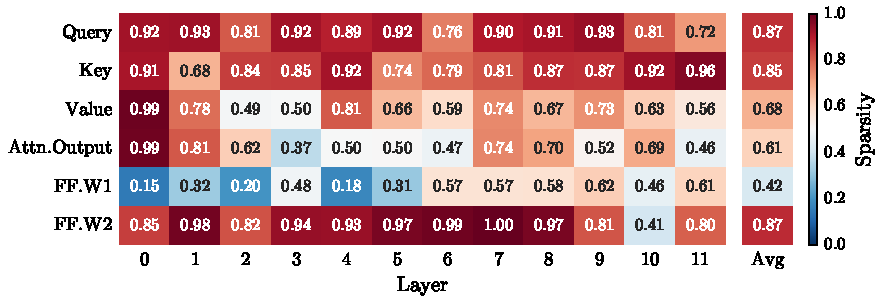
\includegraphics[width=\textwidth]{assets/heatmap.pdf}
  \caption{Sparsity of SpikeLoRA modules in various modules (x-axis) and layers (y-axis) when evaluating the CoLA dataset.}
  \label{fig:sparsity-heatmap}
\end{figure}

Figure \ref{fig:sparsity-heatmap} shows that FF.W1, the intermediate layer, has an average sparsity of 42\%, while FF.W2, the output layer, has an average sparsity of 87\% (about twice FF.W1's sparsity). This indicates that FF.W1 retains richer information than FF.W2. Even though FF.W2 sequentially follows FF.W1, the results align with \cite{skean_layer_2025}, which suggests that intermediate layers encode richer information and enhance performance on downstream tasks.

% \subsubsection{LIF, Gating and Dropout}
% \label{LIFdropout}
% It is also possible to couple SpikeLoRA with dropout (Section \ref{LIFdropout}), allowing for both parametric and non-parametric regularisation. \textcolor{red}{Do a small experiment to compare parametric (SpikeLoRA) vs non-parametric (dropout).}

\section{Conclusion \& Future Work}
\label{conclusion}
By proposing SpikeLoRA, we not only contribute to the realm of parameter-efficient fine-tuning but also show that SNNs are ready to be integrated with current mainstream approaches. Given that SNNs and neuromorphic hardware\footnote{https://brainchip.com} become the new norm, SpikeLoRA will serve as the foundation for the next generation of efficient fine-tuning.

Future work includes designing an adaptive SpikeLoRA that controls the sparsity by dynamically adjusting \(V_t\) during training by means of some scheduler. A more robust approach would be to define a target sparsity hyperparameter with a \(\delta\) tolerance. Furthermore, applying SpikeLoRA to convolutional networks, graph neural networks, and multimodal LLMs presents exciting avenues for exploration. As mentioned in Section \ref{method}, future work includes coupling SpikeLoRA with other methods such as AdaLoRA to further enhance efficiency.

\subsection*{Acknowledgements}
We would like to thank Modal\footnote{https://modal.com} for their funding support.
% We would like to thank Modal\footnote{https://modal.com} and NICIS CHPC\footnote{https://chpc.ac.za} for their funding support.


\bibliography{SpikeGPT}
\bibliographystyle{iclr2026_conference}

\newpage

\appendix

\setcounter{figure}{0}
\setcounter{table}{0}
\setcounter{equation}{0}

\section{Additional Details}
\label{app:a}

\begin{table}[htbp]
  \centering
  \resizebox{0.85\textwidth}{!}{%
    \begin{tabular}{l|cccccc}
    \toprule
    Task & Learning Rate & Batch Size & Epochs & LoRA \(r\) & LoRA Dropout & \(V_t\) \\
    \midrule
    CoLA  & 3e-4 & 32 & 20 & 8 & 0.0 & 0.1 \\
    SST-2 & 8e-4 & 64 & 4  & 8 & 0.0 & 0.1 \\
    MRPC  & 1e-3 & 32 & 20 & 8 & 0.0 & 0.1 \\
    STS-B & 3e-4 & 16 & 8  & 8 & 0.0 & 0.1 \\
    MNLI  & 3e-4 & 64 & 3  & 8 & 0.0 & 0.1 \\
    QNLI  & 3e-4 & 32 & 3  & 8 & 0.0 & 0.1 \\
    RTE   & 1.2e-3 & 32 & 15 & 8 & 0.0 & 0.1 \\
    QQP   & 3e-4 & 64 & 3  & 8 & 0.0 & 0.1 \\
    \bottomrule
    \end{tabular}%
  }
  \caption{Unless otherwise stated, this is our standard hyperparameter setup used to perform experiments.}
  \label{tab:best_params}
\end{table}

\begin{table}[htbp]
    \centering
    \begin{tabular}{lcccc}
    \toprule
    \(V_t\) & Sparsity & MCC & Loss \\
    \midrule
    LoRA & - & \(\mathbf{0.678\pm0.009}\) & \(1.096\pm0.029\) \\
    \midrule
    0.0 & \(0.238\pm0.013\) & \(0.666\pm0.013\) & \(1.156\pm0.037\) \\
    0.01 & \(0.279\pm0.017\) & \(0.665\pm0.015\) & \(1.170\pm0.049\) \\
    0.05 & \(0.352\pm0.011\) & \(0.657\pm0.010\) & \(1.183\pm0.030\) \\
    0.1 & \(0.461\pm0.005\) & \(0.668\pm0.006\) & \(1.124\pm0.014\) \\
    0.25 & \(0.671\pm0.010\) & \(0.666\pm0.008\) & \(1.129\pm0.020\) \\
    0.5 & \(0.835\pm0.007\) & \(0.653\pm0.006\) & \(1.150\pm0.029\) \\
    0.75 & \(0.943\pm0.005\) & \(0.663\pm0.013\) & \(0.942\pm0.093\) \\
    1.0 & \(0.972\pm0.005\) & \(0.652\pm0.013\) & \(0.720\pm0.070\) \\
    1.5 & \(0.989\pm0.004\) & \(0.614\pm0.032\) & \(\mathbf{0.484\pm0.061}\) \\
    2.0 & \(0.997\pm0.003\) & \(0.351\pm0.168\) & \(0.502\pm0.051\) \\
    \bottomrule
    \end{tabular}
    \caption{Evaluation metrics grouped by different \(V_t\) on LoRA and SpikeLoRA (r=8). Values are reported as mean \(\pm\) standard deviation.}
\end{table}

\begin{figure}[htbp]
  \centering
  \includegraphics[width=0.5\textwidth]{assets/gradnorm.pdf}
  \caption{Scatterplot to show the gradnorm relationship between SpikeLoRA (average gradnorm: \(1.554\pm 1.292\)) and LoRA (average gradnorm: \(1.592\pm 1.418\)). The Pearson correlation is 0.678 (p-value: 2.488e-08), indicating a moderately strong correlation between the gradnorms of SpikeLoRA and LoRA.}
  \label{fig:gradnorm}
\end{figure}


\end{document}
